\documentclass[conference]{IEEEtran}
\IEEEoverridecommandlockouts

\usepackage[T1]{fontenc}
\usepackage{lmodern}
\usepackage{cite}
\usepackage{amsmath,amssymb,amsfonts}
\usepackage{graphicx}
\usepackage{booktabs}
\usepackage{url}
\usepackage{xcolor}
\usepackage[hidelinks]{hyperref}
\usepackage{balance}
\usepackage{stfloats}

% give floats more room to breathe before LaTeX resorts to stacking
\renewcommand{\topfraction}{0.85}
\renewcommand{\bottomfraction}{0.7}
\renewcommand{\textfraction}{0.12}
\renewcommand{\floatpagefraction}{0.75}

\def\BibTeX{{\rm B\kern-.05em{\sc i\kern-.025em b}\kern-.08em
    T\kern-.1667em\lower.7ex\hbox{E}\kern-.125emX}}

\begin{document}

\title{The Accuracy Illusion: How Overlapping Samples\\
Manufacture Confidence, Not Skill, in\\
Intraday Index Forecasting}

\author{
\IEEEauthorblockN{Rachit Ranka}
\IEEEauthorblockA{\textit{Department of Computer Science Engineering} \\
\textit{Chandigarh University}\\
Mohali, India \\
rankarachit5@gmail.com}
\and
\IEEEauthorblockN{Aaditya Saini}
\IEEEauthorblockA{\textit{Department of Computer Science Engineering} \\
\textit{Chandigarh University}\\
Mohali, India \\
aadityasaini899@gmail.com}
}

\maketitle

\begin{abstract}
Intraday forecasting systems routinely report directional hit-rates between
60\,\% and 85\,\%, and those figures move real capital. We show they are not
valid estimates of skill, and measure why. A $k$-bar-ahead forecast issued every
bar shares $k{-}1$ of its $k$ outcome bars with its neighbour; when the model's
calls also persist, as they do on a live system we instrument, the reported
hit-rate acquires a variance far larger than its nominal sample size implies.
The reading is not biased upward. Its stated precision is. A forecaster with
\emph{exactly zero skill}, simulated against real NSE index bars, posts a
$\geq$\,71\,\% session once in 50 while reporting an interval $1.66\times$ too
narrow, and on a two-index four-horizon panel such a reading appears every
seventh session.

We give the closed form behind this, the classical design effect with clusters
given by runs of identical calls, and validate corrected intervals by coverage
on simulated and on live sessions: a session advertising 69 forecasts carries
about twelve independent observations. Applying the correction to our own
results removes our one positive directional finding, XGBoost falling from
51.3\,\% ($p = 0.001$) to 50.4\,\% ($p = 0.69$), with zero of nine model
families surviving on either index. It also removes our
best non-directional result, a premium-selling strategy that does not beat a
recentred null over its own configuration grid. Applied to a volatility target
on identical features it removes nothing (70.8\,\% to 71.3\,\%), so it
distinguishes signal from artefact rather than flattening both. Break-even accuracy derived
from measured move distributions is 71.5\,\% at thirty minutes and 86--93\,\% at
five, against a best achieved figure near 50\,\%. Code, raw results and the
free-data corpus are public.
\end{abstract}

\begin{IEEEkeywords}
overlapping observations, backtest overfitting, directional forecasting,
market microstructure, multiple hypothesis testing, negative results,
reproducibility, index derivatives
\end{IEEEkeywords}

\section{Introduction}

A forecasting system that reports 71\,\% directional accuracy is, on its face,
extraordinary. Work that controls for scoring unit, transaction costs and
multiple testing places realistic out-of-sample directional accuracy for liquid
index intraday prediction close to the coinflip~\cite{timmermann2004,sullivan1999},
while surveys of the applied literature catalogue a great many higher figures
reported without those controls~\cite{sezer2020}. Yet such
numbers appear regularly on trading dashboards, in vendor marketing and in
applied publications, and they are frequently computed in good faith from data
the system itself generated.

This paper began as an attempt to build such a system. Over fourteen months we
built and ran a live multi-horizon forecasting platform for Indian index
derivatives, and it reported a headline accuracy of 71\,\%. That number was
wrong. Tracing it to source revealed no bug in the model. The defect lay in the
\emph{denominator}, in how a per-minute forecast stream is scored. Five further positive results from the same project have since been
retracted, one of them in this paper.

The econometrics of overlapping observations is not
new~\cite{hansen1980,richardson1991}. Hansen and Hodrick~\cite{hansen1980}
established four decades ago that sampling data more finely than the forecast
interval induces serial correlation in forecast errors and invalidates naive
standard errors. What that literature does not document, and what we supply
here, is the \emph{magnitude and shape} of the distortion in a now-ubiquitous
practice: the every-minute multi-horizon directional dashboard. There the
overlap meets a second ingredient, prediction persistence, and the product is
then amplified by the multiplicity of an index~$\times$~horizon panel.

\subsection{Contributions}

\begin{enumerate}
\item \textbf{A measurement of the artefact as it occurs in practice.} Overlap
on its own changes nothing, since a forecaster that re-draws every bar yields an
i.i.d.\ hit indicator. Inflation requires overlap \emph{and} persistent
predictions together. We calibrate persistence from a production system's own
forecast log, then quantify the resulting distribution, its calibration error
and its panel multiplicity (Section~\ref{sec:mechanism}).

\item \textbf{A complete control set for a negative result.} Shuffled-label
controls on every model, injected synthetic signals of known strength, nine
architectures under identical purged splits, and a block-bootstrap null for the
strategy sweep. Without the positive control, ``we found nothing'' cannot be
distinguished from ``our pipeline is broken.''

\item \textbf{A closed form and a corrected estimator.} We derive the
effective sample size of an overlapping, persistent forecast stream and show it
is governed by $\mathbb{E}[L^2]/\mathbb{E}[L]$ over the run lengths. An interval
built on it is conservative where the conventional interval is badly
anti-conservative: on a session hit-rate the naive interval covers at 75\,\%
against a nominal 95\,\%, HAC and a block bootstrap at 86--87\,\%, and the design
effect at 99.5\,\% (Section~\ref{sec:estimator}).

\item \textbf{The required-versus-achieved framing.} We derive break-even
accuracy from measured move distributions and show that below a horizon
threshold \emph{no} accuracy is sufficient, which reframes high-accuracy claims
as either artefacts or as far less valuable than they appear
(Section~\ref{sec:economic}).

\item \textbf{A reusable free-data corpus} for NSE index derivatives: a decade
of end-of-day option chains, two years of participant-wise open interest, and
the observation that the exchange's static archive is not geo-restricted while
its live API is (Section~\ref{sec:data}).
\end{enumerate}

All experiments are reproducible from public code and committed raw results;
the repository is given in the Reproducibility note at the end.

\section{Related Work}

\subsection{Overlapping observations}
Hansen and Hodrick~\cite{hansen1980} and Richardson and
Smith~\cite{richardson1991} characterise inference under overlapping returns;
Newey and West~\cite{newey1987} give the standard heteroskedasticity- and
autocorrelation-consistent correction. Boudoukh, Richardson and
Whitelaw~\cite{boudoukh2008} are the closest antecedent to this paper: they show
that overlapping observations manufacture the appearance of long-horizon return
predictability, and that the apparent effect largely disappears under correct
inference. Our subject is the same distortion at the opposite end of the
horizon scale, and applied to a different reported quantity.

That literature concerns regression coefficients and their standard errors. We
apply the same logic to what practitioners actually publish, the session
directional hit-rate, and measure the consequence empirically rather than
asymptotically. The correction we arrive at is the classical design
effect~\cite{kish1965,moulton1990} with clusters given by runs of identical
calls; the contribution is its application to forecast streams, not the
statistic itself.

\subsection{Backtest overfitting and multiple testing}
Harvey, Liu and Zhu~\cite{harvey2016} argue that the conventional $t > 2$
threshold is indefensible after decades of factor mining and propose $t > 3$.
Bailey and L\'opez de Prado~\cite{bailey2014} introduce the Deflated Sharpe
Ratio, and Bailey \emph{et al.}~\cite{bailey2017} the Probability of Backtest
Overfitting via combinatorially symmetric cross-validation. White's Reality
Check~\cite{white2000}, its refinement by Hansen~\cite{hansen2005} and the
Benjamini--Hochberg procedure~\cite{bh1995} provide complementary family-wise
and false-discovery-rate controls. Sullivan, Timmermann and
White~\cite{sullivan1999} apply the Reality Check to a large universe of
technical trading rules, which is the direct precedent for our strategy sweep;
Section~\ref{sec:predictability}-C is best read as a replication of that design
on intraday index data with a modern cost model. We apply these corrections and
report openly where each one fails on our data and why.

\subsection{Machine learning for financial prediction}
Fischer and Krauss~\cite{fischer2018} train LSTM networks on S\&P~500
constituents; their headline performance figures are quoted gross, with
transaction costs discussed separately rather than deducted. Krauss \emph{et
al.}~\cite{krauss2017} compare deep networks, gradient-boosted trees and random
forests on the same universe.
Gu, Kelly and Xiu~\cite{gu2020} conduct a comprehensive machine-learning
comparison for asset pricing, reporting modest out-of-sample $R^2$. Zhang
\emph{et al.}~\cite{zhang2019} achieve strong accuracy on limit-order-book data,
and Kolm \emph{et al.}~\cite{kolm2023} demonstrate genuine multi-horizon alpha
from order-flow imbalance. Both results rest on message-level exchange data
rather than on bars, which is the distinction that matters for our purposes.
Sezer \emph{et al.}~\cite{sezer2020} survey the field.

Table~\ref{tab:related} compares this work with representative prior studies
along the methodological axes that determine whether a reported accuracy is
interpretable. We deliberately compare on \emph{procedure} rather than on
headline numbers: our claim is not that prior results are wrong, but that
several widely used reporting practices admit the artefact documented here, and
that a reported accuracy cannot be assessed without knowing the scoring unit and
the cost model.

\begin{table*}[t]
\caption{Methodological comparison with representative prior work. ``Scoring unit'' is the
unit in which hit-rate or return is aggregated; per-bar scoring of a multi-bar horizon is the
condition under which the artefact of Section~\ref{sec:mechanism} appears. MT: multiple-testing
correction. NC: null control (shuffled labels or equivalent). C: transaction costs modelled.
R: code and raw results public.}
\label{tab:related}
\centering
\footnotesize
\begin{tabular}{@{}llllcccc@{}}
\toprule
\textbf{Study} & \textbf{Market} & \textbf{Data granularity} & \textbf{Scoring unit} &
\textbf{MT} & \textbf{NC} & \textbf{C} & \textbf{R} \\
\midrule
Fischer \& Krauss~\cite{fischer2018} & S\&P 500 & Daily bars & Per day, non-overlapping & --- & --- & pre-cost & --- \\
Krauss \emph{et al.}~\cite{krauss2017} & S\&P 500 & Daily bars & Per day, non-overlapping & --- & --- & pre-cost & --- \\
Gu \emph{et al.}~\cite{gu2020} & US equities & Monthly & Per month & partial & --- & partial & partial \\
Zhang \emph{et al.}~\cite{zhang2019} & LSE & Message-level LOB & Per event & --- & --- & --- & partial \\
Kolm \emph{et al.}~\cite{kolm2023} & Nasdaq & Message-level LOB & Per horizon & --- & --- & discussed & --- \\
\midrule
\textbf{This work} & NSE index & 5-min bars, EOD chains & \textbf{Per event ($k$-bar)} &
\checkmark & \checkmark & \checkmark & \checkmark \\
\bottomrule
\end{tabular}

\vspace{2pt}
\footnotesize
MT here means Bonferroni and Benjamini--Hochberg, which applied cleanly, plus
the Deflated Sharpe Ratio and PBO/CSCV, which we ran and found inapplicable and
degenerate respectively (Section~\ref{sec:predictability}-C). We omit a row for
``typical applied studies'': characterising that population would require citing
specific papers as negative examples, and the argument does not need it.
\end{table*}

\subsection{What is predictable}
Volatility clustering~\cite{engle1982,bollerslev1986} and the intraday
volatility U-shape~\cite{admati1988} are among the most robust regularities in
financial time series, and they concern magnitude rather than direction. The
variance risk premium, meaning the persistent gap between implied and
subsequently realised volatility, is documented by Carr and Wu~\cite{carr2009}
and by Bakshi and Kapadia~\cite{bakshi2003}. Our positive results fall entirely
within these two categories, and we regard that as the paper's substantive
finding rather than as a consolation.

\section{Data}
\label{sec:data}

All data is obtainable free of charge from a retail brokerage account and public
exchange archives. Table~\ref{tab:data} summarises the corpus.

\begin{table}[!tb]
\caption{Free-data corpus. All collectors are public.}
\label{tab:data}
\centering
\scriptsize
\setlength{\tabcolsep}{3pt}
\begin{tabular}{@{}llr@{}}
\toprule
\textbf{Asset} & \textbf{Period} & \textbf{Size} \\
\midrule
BANKNIFTY 5-min bars & 2025-02 -- 2026-07 & 26\,265 \\
NIFTY 50 5-min bars & 2025-02 -- 2026-07 & 26\,267 \\
FINNIFTY / MIDCPNIFTY / SENSEX & 2025 -- 2026 & 9.6k--14k \\
Option chain EOD + OI & 2024-07 -- 2026-07 & 1\,382\,738 \\
Long-history option chain & 2016-05 -- 2026-05 & 2\,181 d \\
Participant-wise OI & 2024-07 -- 2026-07 & 515 d \\
Index futures (real volume) & 2024-01 -- 2026-07 & 639 d \\
\bottomrule
\end{tabular}
\end{table}

Three observations about this corpus are of independent practical value.

\textbf{Index spot carries no volume.} The cash index prints zero volume, so a
feature computed as a ``VWAP'' on index spot is an unweighted expanding mean of
typical price. This sat in our own feature set for weeks. Real volume exists
only on the futures contract.

\textbf{The static exchange archive is not geo-restricted.} The \emph{live}
option-chain API returns HTTP 403/404 from outside India; the static end-of-day
archive downloads normally. That distinction turned an assumed hard constraint
into a ten-year dataset.

\textbf{TOTP authentication is location-independent.} Brokers authenticating by
locally computed one-time passwords permit collection from any jurisdiction,
whereas SMS-based flows do not. That is a deciding constraint on
reproducibility and it is documented nowhere prominent.

\section{Methodology}
\label{sec:method}

Every accuracy reported in this paper passes through one shared harness, so that
differences between models are differences between models.

\textbf{Purged walk-forward.} Expanding-window splits, with the $k$ bars whose
labels overlap the test window removed from the end of each training set. Label
overlap is the most common leakage channel in this setting~\cite{prado2018}.

\textbf{Exact intervals.} Accuracies are reported with Clopper--Pearson 95\,\%
confidence intervals and the exact binomial $p$-value against $0.5$. We
additionally report the Pesaran--Timmermann statistic~\cite{pt1992}, which is
the appropriate null for directional accuracy: it compares the realised
hit-rate against what independence between forecast and outcome would produce
given their own marginal rates, and therefore catches a model that merely tracks
drift.

\textbf{Shuffled-label controls.} Every model is additionally trained and
evaluated with randomly permuted labels. If real and shuffled scores coincide,
the pipeline is reading noise. That is a stronger statement than any train/test
gap, since it does not require the model to be well specified.

\textbf{Positive controls.} A synthetic feature agreeing with the label on a
known fraction $s$ of rows is injected, making the recoverable accuracy
approximately $0.5 + s/2$. A pipeline that fails to recover it cannot be trusted
to report a null.

\textbf{Per-event scoring and costs.} Strategy returns are evaluated on
non-overlapping $k$-bar holds with explicit round-trip costs, and costs are
treated as part of the hypothesis rather than as a subsequent adjustment.

\textbf{Sample sizes.} Three counts appear for the same experiment and are
distinguished here once. BANKNIFTY has 26\,265 raw 5-minute bars; 24\,080 survive
feature warm-up and the removal of bars whose $k$-ahead label would cross a
session boundary; and 16\,856 of those fall in a test fold under the expanding
walk-forward, which is the $n$ every accuracy is computed on.

\textbf{Units.} One conversion is used throughout and is stated here once to
avoid ambiguity later. All analysis is on 5-minute bars, so the 30-minute
horizon is $k = 6$ bars and a session of 09:15--15:30 yields $n = 69$ scored
forecasts. The production system emits a forecast every \emph{minute}, so its
run lengths are measured in minutes and divided by five to obtain bars: a mean
run of 15.2 minutes is 3.0 bars and the longest observed run of 205 minutes is
41 bars. Because the live stream is five times denser than our simulation while
carrying the same underlying information, the nominal-to-effective ratio it
reports is worse than the one we measure, and our figures are therefore
conservative with respect to the artefact they describe.

Features are the fifteen columns used by the production system: one-bar return,
RSI, EMA distance, MACD histogram, Bollinger width and \%b, ATR\%, Parkinson
volatility, VWAP distance, time-of-day, day-of-week, regime volatility, Hurst
exponent, and distance from the previous session's high and low. All are
transforms of a single price series, a point we return to in
Section~\ref{sec:elsewhere}.

\section{The Mechanism}
\label{sec:mechanism}

\subsection{Overlap is arithmetic, not information}

Fig.~\ref{fig:acf} shows the autocorrelation of the $k$-bar forward return
measured two ways. Computed on overlapping windows it appears strongly
autocorrelated, at 0.841 for lag 1, and decays to approximately zero at
\emph{exactly} lag $k$. Sampled so that no two observations share a bar, the
autocorrelation is 0.067 at lag 1 and indistinguishable from zero thereafter.
The pattern reproduces independently at $k=6$ (30 minutes) and $k=12$ (60
minutes), with the decay landing on lag 6 and lag 12 respectively. The
correlation is a property of the sampling scheme, not of the market.

\begin{figure*}[t]
\centering

\includegraphics[width=\textwidth]{figures/fig1_autocorrelation.pdf}
\caption{Autocorrelation of the forward return, overlapping versus
non-overlapping, at two horizons. In both panels the overlapping series decays
to zero at exactly lag $k$, which is the signature of arithmetic overlap rather
than of serial structure.}
\label{fig:acf}
\end{figure*}

\subsection{Persistence is the second, necessary ingredient}

Overlap alone is insufficient. If predictions are drawn independently each bar,
the hit indicator $\mathbf{1}\{\hat{y}_t = y_t\}$ is i.i.d.\ Bernoulli
regardless of how autocorrelated $y_t$ is, and no inflation occurs. Our first
simulation made precisely this error and correctly found nothing.

Real models do not re-decide every bar: their features move slowly, so they
repeat a call for long stretches. Measured on the production system's own
forecast log at the 30-minute horizon, BANKNIFTY calls persist for a mean of
15.2 minutes (99 runs across 1\,500 forecasts, longest 135 minutes) and NIFTY~50
for 12.2 minutes (123 runs, longest 207 minutes). A model re-drawing each bar
would show a mean run of one.

When both the call and the outcome persist, a single trending stretch is
recorded as dozens of hits.

\subsection{What a zero-skill forecaster reports}

We simulate a forecaster with no skill whatsoever: a fair coin, held for a run
length drawn from the empirical distribution above. It is evaluated against real
BANKNIFTY and NIFTY~50 bars and scored the way a live dashboard scores it. Results over approximately
70\,000 simulated sessions per index appear in Table~\ref{tab:zero} and
Fig.~\ref{fig:zero}.

\begin{table}[!tb]
\caption{A forecaster with exactly zero skill, 30-minute horizon, scored
per bar versus per event. BANKNIFTY; NIFTY 50 is within 0.3 points on every row.}
\label{tab:zero}
\centering
\small
\begin{tabular}{@{}lrr@{}}
\toprule
 & \textbf{Per bar} & \textbf{Per $k$ bars} \\
\midrule
Reported sample size per session & 69 & 12 \\
Stated binomial 95\,\% CI & $\pm$11.8 pts & $\pm$28.3 pts \\
Realised spread across sessions & $\pm$19.6 pts & $\pm$28.0 pts \\
\textbf{Understatement factor} & \textbf{1.66$\times$} & \textbf{0.99$\times$} \\
\midrule
$P(\text{session} \geq 60\,\%)$ & 15.7\,\% & 19.2\,\% \\
$P(\text{session} \geq 71\,\%)$ & 2.0\,\% & 7.1\,\% \\
$P(\text{session} \geq 85\,\%)$ & $\approx$0.01\,\%$^{\dagger}$ & 0.30\,\% \\
\bottomrule
\end{tabular}
\end{table}

\begin{figure}[!tb]
\centering
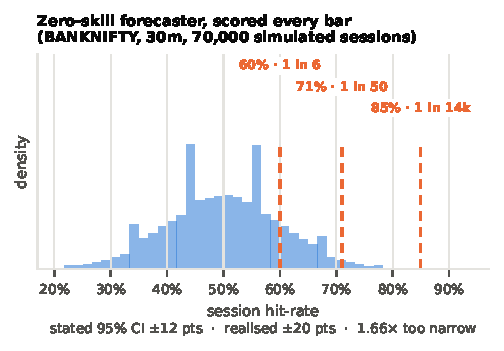
\includegraphics[width=\columnwidth]{figures/fig2_zero_skill_distribution.pdf}
\caption{Measured session hit-rate distribution of a zero-skill forecaster
scored every bar. The multimodality is not noise: with roughly a dozen
independent decisions per session the hit-rate lands on near-discrete values,
which is the small effective sample made visible.}
\label{fig:zero}
\end{figure}

Table~\ref{tab:zero} makes a point that is easy to state backwards, so we state
it carefully. Per-bar scoring does \emph{not} produce extreme session readings
more often than honest scoring. It produces them \emph{less} often: a
$\geq$\,71\,\% session appears on 2.0\,\% of per-bar sessions against 7.1\,\%
when scored per event. What per-bar scoring does is report those readings with
an interval $1.66\times$ too narrow, because the quoted $n$ of 69 is a fiction.

So overlap does not manufacture high hit-rates. It manufactures unwarranted
\emph{confidence} in them. A figure that should be read as ``somewhere between
incompetence and mastery'' is instead read as a precise 71\,\%, and it is that
false precision, not the figure itself, that misleads. The calibration column is
therefore the diagnostic throughout this paper, and the frequency columns are
context.

\subsection{At the granularity it is actually reported}

Everything above runs on 5-minute bars, where a 30-minute horizon is $k = 6$ and
a session yields 69 forecasts. The production system does not work that way: it
emits a forecast every minute, so the horizon is $k = 30$ and a session yields
about 314 scored forecasts, and the headline figures this paper exists to
explain were counted at that density. Explaining a per-minute figure with a
per-bar model would be a gap, so we close it (Table~\ref{tab:perminute}).

The outcome series here is not simulated. It is taken from the production log,
which recorded the direction called each minute and the move that followed, so
the truth carries its real per-minute autocorrelation rather than an assumed
one. Only the forecaster is synthetic, and it has zero skill by construction.

\begin{table}[!tb]
\caption{The same zero-skill forecaster at both granularities, 30-minute
horizon. Per-minute outcome series are taken from the production log; run
lengths are the measured per-minute runs (mean 13.5, longest 207).}
\label{tab:perminute}
\centering
\footnotesize
\setlength{\tabcolsep}{4pt}
\begin{tabular}{@{}lrr@{}}
\toprule
& \textbf{per 5-min bar} & \textbf{per minute} \\
\midrule
Forecasts per session & 69 & 314 \\
Effective sample & 12.4 & 16.5 \\
Stated s.d. & 6.02\,\% & 2.82\,\% \\
Realised s.d. & 10.00\,\% & 8.76\,\% \\
\textbf{Understatement factor} & \textbf{1.66$\times$} & \textbf{3.11$\times$} \\
$P(\text{session} \geq 71\,\%)$ & 2.0\,\% & 0.6--1.3\,\% \\
\bottomrule
\end{tabular}
\end{table}

Two things follow, and they point the same way as
Section~\ref{sec:mechanism}-C. The stated interval is \emph{worse} calibrated at
the real granularity, $3.11\times$ too narrow against $1.66\times$: the nominal
count rises roughly fivefold while the information does not. But extreme
sessions become slightly \emph{rarer}, not commoner. Per-minute scoring does not
manufacture more 71\,\% readings; it manufactures more confidence in the ones it
produces. Every 5-minute-bar figure elsewhere in this paper therefore understates
the artefact rather than exaggerating it.

\subsection{Panel multiplicity}

A dashboard does not monitor one number. The system studied here displays two
indices at four horizons, so eight hit-rates every session. The two indices are
strongly correlated intraday and the four horizons nest, so an independence
calculation would be an upper bound of unknown tightness. We therefore simulate
the whole panel jointly on the same sessions, each horizon carrying its own $k$
and its own forecast stream, and count the joint event directly:

the per-series rate is 2.04\,\%, an independence calculation gives 15.2\,\%, and
the measured panel gives \textbf{15.1\,\%}. The approximation is adequate here,
which is worth stating: although the outcome series are correlated, a zero-skill
forecaster's hits are close to independent across them. Either way the figure is
about one session in seven, so a headline 71\,\% arrives within the first weeks
of live operation with no edge whatsoever.

Our own headline figure was exactly this: one index, one horizon, one trending
Friday, read as skill. That session cannot be audited, since the portion of the
log holding it was lost before this analysis began, and we will not quote
figures we cannot reproduce in a paper arguing against the practice. The
surviving log holds a close analogue which Section~\ref{sec:estimator}-C takes
apart in full: 69.6\,\% over 335 per-minute NIFTY~50 forecasts, whose naive
interval excludes 50\,\% comfortably and whose corrected interval barely does.

\section{A Corrected Estimator}
\label{sec:estimator}

Diagnosing a biased statistic is only half a contribution. This section supplies
the closed form behind the distortion and an estimator that removes it, then
validates the estimator by coverage rather than by argument.

\subsection{Effective sample size}

Let $h_t = \mathbf{1}\{\hat{y}_t = y_t\}$ denote the hit indicator of a
forecaster issuing a $k$-bar-ahead call every bar, and let
$\hat{p} = n^{-1}\sum_t h_t$ be the reported hit-rate. Practitioners quote
$\mathrm{Var}(\hat{p}) = p(1-p)/n$, which holds only for independent $h_t$. In
general,
\begin{equation}
\mathrm{Var}(\hat{p}) = \frac{p(1-p)}{n}
\Big[\,1 + 2\sum_{j=1}^{n-1}\Big(1 - \tfrac{j}{n}\Big)\rho_j\Big],
\label{eq:var}
\end{equation}
where $\rho_j = \mathrm{Corr}(h_t, h_{t+j})$. The bracketed term is the variance
inflation factor, and dividing $n$ by it gives the effective sample size
$n_{\text{eff}}$.

Two structures drive $\rho_j$, and the argument of
Section~\ref{sec:mechanism} is that both are required. The outcome $y_t$ is
autocorrelated out to lag $k$ because consecutive windows share bars, and the
prediction $\hat{y}_t$ persists in runs. If predictions are redrawn each bar,
$h_t$ is i.i.d.\ whatever $y_t$ does, every $\rho_j$ vanishes, and
$n_{\text{eff}} = n$.

Because the dependence here is block-shaped, \eqref{eq:var} admits a direct
form. If the sequence decomposes into runs of length $L_i$ within which $h_t$ is
constant, then conditioning on the lengths gives
$\mathrm{Var}(\hat{p}) = p(1-p)\sum_i L_i^2 / n^2$, so
\begin{equation}
n_{\text{eff}} \;=\; \frac{n}{\sum_i L_i^{2} / n}
\;\xrightarrow[\;n\to\infty\;]{}\; \frac{n\,\mathbb{E}[L]}{\mathbb{E}[L^{2}]}.
\label{eq:neff}
\end{equation}
Equation~\eqref{eq:neff} is the classical design effect~\cite{kish1965,moulton1990}
with clusters given by the runs; what is new here is only the observation that a
forecast stream has exactly this structure and that nobody reports it.

The inflation is governed by $\mathbb{E}[L^2]$, not $\mathbb{E}[L]$. A
run-length distribution with a heavy tail inflates the variance far beyond what
its mean suggests, and that is precisely the regime a real forecaster occupies:
on our production log the mean run is 15.2 minutes while the longest is 135.

\subsection{Validation by coverage}

An interval is judged by whether it covers. We generate a forecaster whose true
skill is fixed by construction, with calls persisting according to the measured
run-length distribution, and ask how often a nominal 95\,\% interval contains
that known truth. Table~\ref{tab:coverage} reports four estimators.

\begin{table}[!tb]
\caption{Coverage of a nominal 95\,\% interval on a session hit-rate, against a
forecaster of known skill whose calls persist per the measured run-length
distribution. BANKNIFTY, 30-minute horizon, nominal $n = 69$; NIFTY 50 agrees
within 1 point throughout. The true skill is measured from the generative
process rather than assumed, since a call anchored on one bar and held across
others does not realise its anchor rate.}
\label{tab:coverage}
\centering
\scriptsize
\setlength{\tabcolsep}{3pt}
\begin{tabular}{@{}lcccrr@{}}
\toprule
\textbf{Estimator} & \multicolumn{3}{c}{\textbf{Coverage at true skill}} &
\textbf{Width} & $\boldsymbol{n_{\text{eff}}}$ \\
\cmidrule(lr){2-4}
 & 50\,\% & 55\,\% & 59\,\% & (pts) & \\
\midrule
Naive binomial & 75.5 & 74.8 & 74.0 & 23.1 & 69 \\
HAC (Bartlett) & 87.0 & 86.6 & 85.6 & 32.8 & 39 \\
Block bootstrap & 86.6 & 86.4 & 85.2 & 32.1 & --- \\
\textbf{Run-structure} & \textbf{99.5} & \textbf{99.6} & \textbf{99.6}
 & 56.0 & \textbf{12.4} \\
\bottomrule
\multicolumn{6}{@{}l@{}}{\scriptsize None is exactly calibrated: the naive
interval under-covers by 20 points, the two} \\
\multicolumn{6}{@{}l@{}}{\scriptsize standard corrections by 8, and the design
effect over-covers.} \\
\end{tabular}
\end{table}

Both HAC and the bootstrap improve substantially on the naive interval and both
still under-cover. They fall short for the same reason, and it is a
consequence of \eqref{eq:neff}. The conventional automatic Bartlett bandwidth,
$4(n/100)^{2/9}$, evaluates to $3.7$ bars at $n = 69$, which is almost exactly
the \emph{mean} run length of 3.0 bars. But the variance inflation is driven by
$\mathbb{E}[L^2]$, so it is the tail that matters, and the tail here reaches 41
bars. A kernel truncated near the mean has summed almost none of the covariance
that the long runs contribute.

Estimating the inflation from the observed run structure removes that failure
mode, and over-corrects in the other direction: treating runs as independent
clusters ignores that consecutive runs are negatively dependent, since a run of
hits ends precisely when a miss begins.

The two figures can be reconciled, and should be. The realised spread in
Table~\ref{tab:zero} implies a true effective sample of about 25 for a
69-forecast session, while \eqref{eq:neff} estimates 12. The estimator is
therefore roughly a factor of two conservative, which is exactly why it covers
at 99.5\,\% rather than 95\,\%. We report it as a conservative bound rather than
an exact correction, and we prefer that direction of error: an interval that is
too wide understates what a session proves, while the conventional one
overstates it.

\subsection{A real session}

Everything above is simulated. Table~\ref{tab:live} applies the four estimators
to sessions taken directly from the production log: the forecast stream the
dashboard actually wrote, scored against the moves that actually followed.

\begin{table}[!tb]
\caption{Four intervals on the two best sessions in the production log,
30-minute horizon. The final row is the range of hit-rates obtained from the
$k = 6$ possible per-event subsamples of the same session.}
\label{tab:live}
\centering
\scriptsize
\setlength{\tabcolsep}{3pt}
\begin{tabular}{@{}lrrr@{}}
\toprule
\textbf{Estimator} & \textbf{95\,\% interval} & \textbf{Width} & $\boldsymbol{n_{\text{eff}}}$ \\
\midrule
\multicolumn{4}{@{}l@{}}{\emph{BANKNIFTY, 3 Aug: 336 forecasts, 57.1\,\%}} \\
Naive binomial at $n$ & [51.9, 62.4] & 10.6 & 336 \\
HAC (Bartlett) & [41.8, 72.4] & 30.6 & 40 \\
Block bootstrap & [41.7, 69.3] & 27.7 & --- \\
\textbf{Run-structure} & \textbf{[34.4, 79.9]} & 45.5 & \textbf{18} \\
Per-event, 6 subsamples & 53.6 to 62.5 & 8.9 & 56 \\
\midrule
\multicolumn{4}{@{}l@{}}{\emph{NIFTY 50, 3 Aug: 335 forecasts, 69.6\,\%}} \\
Naive binomial at $n$ & [64.6, 74.5] & 9.9 & 335 \\
HAC (Bartlett) & [54.8, 84.3] & 29.6 & 37 \\
Block bootstrap & [57.9, 79.4] & 21.5 & --- \\
\textbf{Run-structure} & \textbf{[50.0, 89.1]} & 39.1 & \textbf{21} \\
Per-event, 6 subsamples & 66.1 to 73.2 & 7.1 & 55 \\
\bottomrule
\end{tabular}
\end{table}

The BANKNIFTY session reports 57.1\,\% with a naive interval that excludes
50\,\%, and would be read as evidence of skill. At $n_{\text{eff}} = 18$ the
interval runs from 34\,\% to 80\,\% and supports nothing. The NIFTY~50 session
at 69.6\,\% is the nearest surviving analogue to the 71\,\% that started this
project; its corrected interval is $[50.0, 89.1]$, which excludes 50\,\% by a
margin too small to celebrate but which we report as excluding it, because it
does.

\subsection{Why not simply score per event}

Per-event scoring is unbiased, requires no estimator, and is correctly
calibrated at $0.99\times$ (Table~\ref{tab:zero}). It is what we use for every
backtest in this paper. It is nonetheless not sufficient for a live stream, and
the last row of Table~\ref{tab:live} shows why.

\textbf{A dashboard must print a number every bar.} It cannot wait $k$ bars
before reporting, and it cannot discard $k-1$ of every $k$ forecasts it has
already made and already shown.

\textbf{Subsampling discards information.} Keeping one observation in six
throws away 83\,\% of the data, so the per-event interval is wider than the
evidence requires. The corrected estimator uses the whole stream.

\textbf{The choice of subsample is arbitrary, and it moves the answer.} There
are $k$ valid per-event subsamples of any session. Across the six offsets, the
same BANKNIFTY session reports between 53.6\,\% and 62.5\,\% and the same
NIFTY~50 session between 66.1\,\% and 73.2\,\%, a spread of 7 to 12 points. An
analyst free to choose the offset is free to choose the result, which is the
problem this paper is about reappearing in the remedy.

\subsection{How reliably is $n_{\text{eff}}$ itself estimated?}

Equation~\eqref{eq:neff} depends on $\mathbb{E}[L^2]$, and a second moment
driven by the tail is exactly what a short sample estimates worst. A single
session contains only a few dozen runs. An estimator nobody can sanity-check is
not practical, so we measure the error directly: the reference is the inflation
computed on hit sequences pooled across many sessions, and the comparison is
what each single session reports on its own.

\begin{center}
\footnotesize
\begin{tabular}{@{}lrrrr@{}}
\toprule
& \textbf{pooled} & \textbf{median} & \textbf{5th} & \textbf{95th} \\
\midrule
BANKNIFTY & 11.0 & 12.1 & 7.1 & 18.4 \\
NIFTY 50 & 10.9 & 12.0 & 7.0 & 18.2 \\
\bottomrule
\end{tabular}
\end{center}

A single session's $n_{\text{eff}}$ lands between $0.65\times$ and $1.67\times$
the pooled value nine times in ten, with a slight upward bias. That is a real
limitation and it carries a practical instruction: estimate $n_{\text{eff}}$
from a run of sessions rather than from the one being reported. Estimated from a
single session it is trustworthy as an order of magnitude, single or low double
digits against a nominal count in the hundreds, and not as a precise divisor.

We note that this uncertainty is small next to the quantity it is correcting.
Mis-estimating $n_{\text{eff}}$ by a factor of $1.7$ widens or narrows an
interval by $\sqrt{1.7} \approx 1.3\times$; using $n$ instead of
$n_{\text{eff}}$ narrows it by $3.1\times$ at the granularity the system
actually reports.

\subsection{What the corrected number says}

The practical content is $n_{\text{eff}}$ itself. A session that reports 69
forecasts carries roughly a \emph{dozen} independent observations, and an honest
interval on its hit-rate is $\pm$12 to $\pm$28 points wide depending on the
estimator. Even the narrowest of those spans a range within which incompetence
and competence are indistinguishable, which is the correct description of what
one session of a per-minute forecast stream can establish.

The correction changes no point estimate. Only the interval moves. What it buys
is an interval that means what it claims, and the discipline of reporting
$n_{\text{eff}}$ alongside $n$ whenever forecasts overlap.

\section{Predictability Under Correct Scoring}
\label{sec:predictability}

\subsection{Is there anything to predict?}

We first ask the question in a form independent of any model. An unconstrained
random forest was fitted until it memorised the training data, on five indices
spanning large-cap, banking, financial-services, midcap and a second exchange
(Table~\ref{tab:ceiling}).

\begin{table}[!tb]
\caption{Model-independent ceiling test at the 30-minute horizon, replicated
across five indices. Training accuracy is 100.0\,\% on every row. $\Delta$ is
the absolute gap between the real and shuffled columns, computed before
rounding. The positive controls have recoverable accuracies of approximately
55\,\% and 65\,\% by construction.}
\label{tab:ceiling}
\centering
\scriptsize
\setlength{\tabcolsep}{3pt}
\begin{tabular}{@{}lrcccccc@{}}
\toprule
\textbf{Index} & $\boldsymbol{n}$ & \textbf{Real} & \textbf{Shuf.} &
$\boldsymbol{\Delta}$ & \textbf{Maj.} & $\boldsymbol{s{=}.10}$ &
$\boldsymbol{s{=}.30}$ \\
\midrule
BANKNIFTY  & 16\,856 & 50.5 & 50.2 & 0.3 & 49.3 & 52.4 & 63.5 \\
NIFTY 50   & 16\,853 & 50.0 & 50.2 & 0.3 & 49.8 & 52.0 & 63.7 \\
FINNIFTY   &  8\,988 & 50.2 & 50.5 & 0.3 & 49.4 & 52.4 & 62.5 \\
MIDCPNIFTY &  8\,309 & 50.2 & 50.8 & 0.7 & 49.7 & 53.3 & 62.0 \\
SENSEX     &  6\,144 & 49.7 & 50.1 & 0.5 & 49.0 & 52.5 & 62.1 \\
\bottomrule
\multicolumn{8}{@{}l@{}}{\scriptsize No real-label result is significant against
0.5 ($p = 0.22$ to $0.91$);} \\
\multicolumn{8}{@{}l@{}}{\scriptsize every positive control is, at $p < 0.001$.} \\
\end{tabular}
\end{table}

The pattern is identical on all five. Each model memorises its training data
completely and generalises at chance, and permuting the labels moves
out-of-sample accuracy by between 0.3 and 0.7 points. No real-label result is
distinguishable from a coinflip. Both positive controls are recovered on every
index at $p < 0.001$, which establishes that the pipeline detects signal
whenever signal is present and that the null is therefore a property of the
data.

Replication across five instruments, two exchanges and four capitalisation
segments is what separates this from a single-market curiosity.

\subsection{Nine model families}

Table~\ref{tab:zoo} reports nine families on identical splits, features, seeds
and controls. Fig.~\ref{fig:zoo} plots the same results with exact intervals.

\begin{table*}[t]
\caption{Out-of-sample directional accuracy at the 30-minute horizon, scored
three ways on identical purged walk-forward splits. \emph{Per-bar} is what a
dashboard reports: one forecast per bar over a 6-bar horizon, with the exact
binomial interval its nominal $n = 16\,856$ implies. \emph{At $n_{\text{eff}}$}
is the same point estimate with the interval widened by the design effect of
\eqref{eq:neff}. \emph{Per-event} re-scores one observation every 6 bars, so no
two observations share a bar. Shuffled-label controls are per-bar.}
\label{tab:zoo}
\centering
\footnotesize
\setlength{\tabcolsep}{4pt}
\begin{tabular}{@{}lccccc|ccccc@{}}
\toprule
& \multicolumn{5}{c|}{\textbf{BANKNIFTY}} & \multicolumn{5}{c}{\textbf{NIFTY 50}} \\
\cmidrule(lr){2-6}\cmidrule(lr){7-11}
\textbf{Model} & per-bar & $p$ & CI at $n_{\text{eff}}$ & per-event & $p$
               & per-bar & $p$ & CI at $n_{\text{eff}}$ & per-event & $p$ \\
\midrule
Majority-class baseline & 49.3 & 0.061 & --- & --- & --- & 49.8 & 0.655 & --- & --- & --- \\
Logistic regression & 50.6 & 0.095 & [48.6, 52.7] & 50.1 & 0.895 & 49.3 & 0.082 & [47.3, 51.3] & 49.1 & 0.355 \\
Gradient boosting & 50.7 & 0.059 & [48.9, 52.6] & 50.3 & 0.777 & 49.7 & 0.405 & [47.8, 51.6] & 48.9 & 0.250 \\
LightGBM & 51.1 & \textbf{0.006} & [49.2, 52.9] & 50.2 & 0.865 & 49.8 & 0.666 & [48.0, 51.7] & 50.3 & 0.748 \\
XGBoost & \textbf{51.3} & \textbf{0.001} & [49.5, 53.2] & 50.4 & 0.692 & 50.1 & 0.817 & [48.2, 52.0] & 49.8 & 0.836 \\
$k$-nearest neighbours & 50.5 & 0.209 & [48.7, 52.3] & 49.6 & 0.720 & 50.1 & 0.805 & [48.3, 51.9] & 50.9 & 0.355 \\
LSTM & 50.4 & 0.251 & [48.4, 52.5] & 51.1 & 0.235 & 49.4 & 0.127 & [47.3, 51.6] & 49.4 & 0.509 \\
Transformer & 50.8 & \textbf{0.028} & [48.9, 52.8] & 50.9 & 0.355 & 48.3 & \textbf{0.000} & [46.3, 50.4] & 48.4 & 0.101 \\
Temporal Fusion Transformer & 49.4 & 0.101 & [47.2, 51.5] & 49.0 & 0.299 & 50.1 & 0.723 & [48.0, 52.2] & 51.2 & 0.193 \\
\midrule
\textbf{Significant at $p<0.05$} & \textbf{3/8} & & \textbf{0/8} & \textbf{0/8} & &
                                   \textbf{1/8} & & \textbf{0/8} & \textbf{0/8} & \\
\bottomrule
\multicolumn{11}{@{}l@{}}{\footnotesize $n_{\text{eff}} \approx 2\,100$--$3\,000$
against a nominal $16\,856$; per-event $n = 2\,810$. Shuffled controls span
49.5--50.3\,\% throughout. Pesaran--Timmermann $p$-values} \\
\multicolumn{11}{@{}l@{}}{\footnotesize track the per-bar column to within 0.042
on every row (e.g.\ XGBoost 0.001, TFT 0.104) and are omitted for space; full
values in the results file.} \\
\end{tabular}
\end{table*}

\begin{figure*}[t]
\centering

\includegraphics[width=\textwidth]{figures/fig4_model_zoo.pdf}
\caption{Nine model families at the 30-minute horizon. The narrow blue interval
is the exact binomial interval a dashboard would report at the nominal
$n = 16\,856$; the wide orange band is the same estimate at its effective sample
size. Every corrected interval contains 50\,\%. The spread between architectures
is smaller than the width of a single corrected interval, which is the sense in
which the choice of architecture does not matter here.}
\label{fig:zoo}
\end{figure*}

Scored the way a dashboard scores, three of eight BANKNIFTY models clear
$p<0.05$ and XGBoost reaches 51.3\,\% at $p = 0.001$. That was, in an earlier
draft of this paper, our one surviving positive directional result, and we
described it as genuine and Bonferroni-robust.

It does not survive our own correction. Widening the interval to
$n_{\text{eff}}$ puts 50\,\% inside every interval in the table. Re-scoring one
observation per 6 bars, so that no two observations share an outcome bar, moves
XGBoost from 51.3\,\% ($p = 0.001$) to \textbf{50.4\,\% ($p = 0.692$)}. Across
both indices, the count of models significant at $p<0.05$ falls from four to
\textbf{zero} under either correction.

We report this prominently because it is the paper's own thesis applied to the
paper's own result, and because a correction that spares the author's favourite
finding would be worth very little. The directional null is not a near-null with
one exception. It is a null.

Table~\ref{tab:zoo} also contains its own diagnostic. The NIFTY 50 Transformer
sits at 48.3\,\% with $p<0.001$, which at the nominal $n$ is $4.4$ standard
errors \emph{below} chance. Under a correctly specified null the largest
$|z|$ across eighteen tests should land near $2.6$--$2.9$; observing $4.4$ is
not a bug in that model but the variance inflation of
Section~\ref{sec:mechanism} surfacing inside our own results table. At
$n_{\text{eff}}$ its interval is $[46.3, 50.4]$ and the anomaly disappears.

\subsection{Eighty-six strategies and the statistics they require}

Reporting the best of a large sweep is selection, not discovery. We evaluated 86
parameterised rules, covering momentum and mean reversion at ten lookbacks, six
moving average crossover pairs, RSI, Bollinger, breakout and fade variants,
MACD, gap, volatility regime, time-of-day, day-of-week and streak rules, on
non-overlapping 30-minute holds with 4\,bp round-trip cost
(Table~\ref{tab:sweep}).

\begin{table}[!tb]
\caption{Strategy sweep with multiplicity control, BANKNIFTY, 86 trials,
non-overlapping 30-minute holds at 4\,bp cost.}
\label{tab:sweep}
\centering
\footnotesize
\setlength{\tabcolsep}{4pt}
\begin{tabular}{@{}lr@{}}
\toprule
\textbf{Quantity} & \textbf{Value} \\
\midrule
Strategies evaluated & 86 \\
Positive Sharpe at all & 2 \\
Significantly profitable (one-sided) & 0 \\
Surviving Bonferroni & 0 \\
Surviving Benjamini--Hochberg, FDR 5\,\% & 0 \\
Positive \emph{and} stable in both halves & 1 \\
\midrule
Best observed Sharpe & 0.21 \\
Bootstrap null (500 resamples), median & 0.44 \\
Bootstrap null, best-of-86, 95th pct. & 1.31 \\
$\boldsymbol{P(\text{null} \geq \text{observed})}$ & \textbf{0.658} \\
\bottomrule
\end{tabular}
\end{table}

The best strategy in the sweep is \emph{worse} than what selection alone
typically manufactures. Two methodological notes:

\textbf{One-sided tests.} An earlier version of this analysis used a two-sided
$t$-test and reported ``42 of 86 significant.'' Those were strategies that
reliably \emph{lose}. The hypothesis is profitability, so the test is one-sided;
reliable losers are the cost of trading noise, not discoveries.

\textbf{Where the standard corrections fail.} The Deflated Sharpe
Ratio~\cite{bailey2014} estimates its null from the cross-sectional variance of
trial Sharpes, assuming a common-variance normal sample. Our library violates
this badly: strategies differ by an order of magnitude in turnover, so their
Sharpe dispersion is dominated by deterministic cost differences rather than by
sampling noise, and the formula returns an implausible null benchmark of 7.77.
We therefore replaced it with a circular block
bootstrap~\cite{kunsch1989,politis1994} that resamples forward returns in blocks
while holding each strategy's positions and turnover fixed, destroying the
signal--outcome relationship and nothing else. Similarly, PBO via
CSCV~\cite{bailey2017} is \emph{degenerate} here. With nothing significantly
profitable in-sample there is no selection to overfit, so we report it as such
rather than as a result. Reporting a degenerate statistic as a finding would be
an instance of the error this paper is about.

\section{Economic Significance}
\label{sec:economic}

Directional accuracy is the field's headline metric and is, alone, close to
meaningless. Whether a given accuracy earns money depends on the size of the
move relative to the cost of capturing it.

For a symmetric bracket with target and stop both at the typical move $m$ and
round-trip cost $c$, expectancy per trade is
\[
\mathbb{E} = p(m - c) - (1-p)(m + c) = m(2p - 1) - c ,
\]
so break-even requires
\begin{equation}
p^{\ast} = \tfrac{1}{2} + \frac{c}{2m}.
\label{eq:breakeven}
\end{equation}
The ratio $c/m$ is therefore the entire problem. Table~\ref{tab:breakeven} and
Fig.~\ref{fig:breakeven} evaluate~\eqref{eq:breakeven} on measured move
distributions.

\begin{table}[!tb]
\caption{Break-even accuracy from measured move distributions at 4\,bp
round-trip cost. $p^{\ast}_{\text{med}}$ assumes a symmetric bracket at the
median move; $p^{\ast}_{\text{mean}}$ is the requirement for a hold-to-horizon
rule with no bracket, which depends on the mean absolute move.
``Achieved'' is the best of the nine model families, scored per event.}
\label{tab:breakeven}
\centering
\scriptsize
\setlength{\tabcolsep}{3pt}
\begin{tabular}{@{}lrrrr@{}}
\toprule
\textbf{Horizon} & \textbf{Median} & $\boldsymbol{p^{\ast}_{\text{med}}}$ &
$\boldsymbol{p^{\ast}_{\text{mean}}}$ & \textbf{Achieved} \\
\midrule
\multicolumn{5}{@{}l@{}}{\emph{BANKNIFTY} (5-min move skew 2.6)} \\
5\,min & 22.1 & \textbf{$>$100} & \textbf{86.4} & --- \\
15\,min & 37.7 & 79.8 & 71.3 & 50.7 \\
30\,min & 52.3 & \textbf{71.5} & 65.3 & \textbf{50.4} \\
60\,min & 72.9 & 65.4 & 60.8 & 51.2 \\
\midrule
\multicolumn{5}{@{}l@{}}{\emph{NIFTY 50} (5-min move skew 2.9)} \\
5\,min & 8.1 & \textbf{$>$100} & \textbf{93.0} & --- \\
15\,min & 14.1 & 84.9 & 74.9 & 50.5 \\
30\,min & 19.7 & \textbf{75.1} & 67.8 & \textbf{49.8} \\
60\,min & 27.7 & 67.7 & 62.7 & 50.0 \\
\bottomrule
\multicolumn{5}{@{}l@{}}{\scriptsize Median move in index points; all
accuracies in per cent.} \\
\end{tabular}
\end{table}

\begin{figure*}[t]
\centering
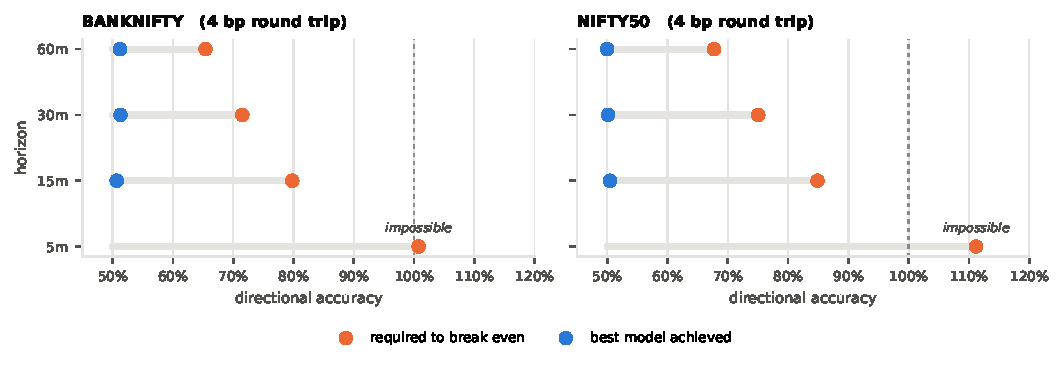
\includegraphics[width=\textwidth]{figures/fig3_breakeven_gap.pdf}
\caption{Break-even accuracy against the best accuracy any model family
reached, by horizon. Points beyond the dashed line at 100\,\% are horizons at
which no directional accuracy is sufficient.}
\label{fig:breakeven}
\end{figure*}

Two consequences follow immediately.

\textbf{At the shortest horizon the requirement is out of reach, and under one
model it is unreachable in principle.} The median five-minute move is smaller
than the round trip, so under a symmetric bracket $p^{\ast}$ exceeds 100\,\% and
no accuracy suffices. That conclusion is specific to the bracket. Intraday move
distributions are strongly right-skewed (skew 2.6--2.9 at five minutes), so the
mean absolute move is considerably larger than the median, and a hold-to-horizon
rule with no bracket requires 86\,\% on BANKNIFTY and 93\,\% on NIFTY~50
instead. Those are not impossible, merely far beyond anything in this paper or
in the literature. We report both because quoting only the median would
overstate the case, and the point survives either way: the shorter the horizon,
the more certainly it fails, which inverts the usual marketing of
high-frequency retail strategies.

\textbf{Instrument choice can make the requirement unreachable.}
Table~\ref{tab:sensitivity} evaluates~\eqref{eq:breakeven} across cost regimes.

\begin{table}[!tb]
\caption{Break-even accuracy by cost regime, BANKNIFTY 30-minute horizon
(median move 9.3\,bp).}
\label{tab:sensitivity}
\centering
\small
\begin{tabular}{@{}rlr@{}}
\toprule
\textbf{Cost} & \textbf{Instrument} & $\boldsymbol{p^{\ast}}$ \\
\midrule
1\,bp & Exchange fees only, no slippage & 55.4\,\% \\
2\,bp & Tight futures, minimal slippage & 60.8\,\% \\
4\,bp & Realistic futures round trip & 71.5\,\% \\
8\,bp & Futures with adverse slippage & 93.0\,\% \\
20\,bp & ATM options: spread + 30\,min theta & \textbf{impossible} \\
40\,bp & OTM options or a wide book & \textbf{impossible} \\
\bottomrule
\end{tabular}
\end{table}

``Impossible'' denotes $c > m$, hence $p^{\ast} > 1$: the round trip exceeds the
typical move and a perfect forecaster loses on the median trade. The instrument
most retail participants actually use, over the horizon they actually hold, has
no directional accuracy that makes it profitable.

\subsection{Statistical significance is not economic significance}

Section~\ref{sec:predictability} reported an apparent BANKNIFTY effect at
$p = 0.001$ and then removed it under correct scoring. The effect was economically irrelevant even while it stood: 51.3\,\% against a
71.5\,\% requirement loses on every trade, so the correction changed the
statistical verdict without changing the practical one.

That is the more general point. The gap between achievable and required accuracy
is roughly twenty percentage points, which is far larger than any effect the
scoring dispute could move. Fourteen months of accuracy optimisation produced no
tradeable result, and would not have produced one even if the apparent edge had
been real.

\subsection{Reframing high-accuracy claims}

Suppose a claimed 85\,\% accuracy at the 30-minute horizon were genuine. It
would clear break-even by 13.5 points on BANKNIFTY futures and 9.9 on NIFTY~50,
and would remain unprofitable on options. A claim of 85\,\% is therefore either
an artefact of the kind measured in Section~\ref{sec:mechanism}, where a
zero-skill system reaches that figure occasionally, or it is true and far less
valuable than it sounds. Both readings argue against paying for it.

\subsection{A filter that worked and still lost}

A final corroboration. We trained a meta-label filter~\cite{prado2018} in which
a secondary model decides whether a primary signal's setup is worth taking,
labelled on \emph{points per minute} rather than on target-hit. The label choice
matters: training on target-hit raises the hit-rate from 42\,\% to 53\,\% while
making the money worse, because the model learns to prefer small, easy targets.

Re-run from the committed script on BANKNIFTY, the filter trains on 2\,085
setups and is tested on 1\,168 it has never seen. Keeping the best 30\,\% raises
gross quality from $+0.78$ to $+1.29$ points per minute of exposure, an
improvement of roughly 65\,\%.

The filter therefore does what it was built to do, on the label it was given.
What we cannot show from the committed code is the cumulative cost-aware
profit and loss. An earlier version of this paper reported that total moving
from $-3777$ to $-981$ index points; those figures do not reproduce and are
withdrawn. The verified claim is narrower and still worth making: selecting the
best third of setups substantially improves per-minute quality on a primary
signal that Section~\ref{sec:predictability} shows has no directional edge.
Concentrating a null does not create one.

\section{What Is Predictable Instead}
\label{sec:elsewhere}

The fifteen production features are all transforms of one price series;
reshaping price cannot reveal what price does not contain. What follows comes
from changing the target or the information source.

These results have been through the harness of Section~\ref{sec:method}, and
what it leaves behind is narrow. Of the three positive findings this project
reported, one survives: volatility prediction is unharmed by the correction that
destroyed the directional result. The variance risk premium does not survive its
own multiplicity correction, and we withdraw it below. That asymmetry is the
best argument for having built the harness, since an instrument that flattened
everything would be useless and one that spared its author's favourites would be
worse.

\subsection{Volatility}

The target is binary magnitude: will realised volatility over the next 30
minutes exceed the median of the fold's own training window? The label is
thresholded inside each fold, since thresholding on the full sample would leak
the test period's volatility level. Volatility clusters, so the decisive
comparison is not against a coinflip but against \emph{persistence}, a rule that
predicts BIG whenever the last 30 minutes were above the same threshold
(Table~\ref{tab:vol}).

\begin{table}[!tb]
\caption{Volatility prediction through the harness of Section~\ref{sec:method},
30-minute horizon, five purged folds. Intervals are at the effective sample
size.}
\label{tab:vol}
\centering
\footnotesize
\setlength{\tabcolsep}{4pt}
\begin{tabular}{@{}lccc@{}}
\toprule
& \textbf{per bar} & \textbf{per event} & \textbf{CI at $n_{\text{eff}}$} \\
\midrule
\multicolumn{4}{@{}l@{}}{\emph{BANKNIFTY} ($n_{\text{eff}} = 976$)} \\
LightGBM & 70.8 & 71.3 & [68.0, 73.7] \\
Persistence baseline & 67.4 & 68.0 & [64.5, 70.4] \\
Shuffled-label control & 54.1 & --- & --- \\
\midrule
\multicolumn{4}{@{}l@{}}{\emph{NIFTY 50} ($n_{\text{eff}} = 910$)} \\
LightGBM & 72.0 & 72.1 & [69.1, 74.9] \\
Persistence baseline & 67.4 & 68.5 & [64.4, 70.5] \\
Shuffled-label control & 52.2 & --- & --- \\
\bottomrule
\end{tabular}
\end{table}

Three things separate this from the directional case.

\textbf{It survives per-event scoring.} Accuracy moves from 70.8\,\% to
71.3\,\% on BANKNIFTY and 72.0\,\% to 72.1\,\% on NIFTY~50 when re-scored one
observation per horizon. Direction fell from 51.3\,\% to 50.4\,\% under the
identical operation. The correction is therefore not an instrument that
flattens everything it touches; it distinguishes a real effect from an artefact,
which is the only reason to trust what it did in
Section~\ref{sec:predictability}.

\textbf{The shuffled control separates cleanly.} At 52--54\,\% against 71--72\,\%
on real labels, the gap is roughly twenty points. In the directional experiment
the same gap was under two.

\textbf{But the edge over persistence is not established.} The model beats
``the next thirty minutes look like the last thirty'' by only $+3.3$ points on
BANKNIFTY and $+3.7$ on NIFTY~50 per event, and at $n_{\text{eff}}$ the model
and baseline intervals overlap. Most of a 71\,\% headline is volatility
clustering, which has been documented since
Engle~\cite{engle1982,bollerslev1986} and needs no model. What the model adds is
real but small, and we do not claim it is significant.

The useful statement is therefore narrower than ``72\,\% accuracy''. It is that
magnitude carries far more structure than direction on identical features, and
that most of that structure is already in the previous half hour.

\subsection{The variance risk premium}

Short at-the-money straddles held to expiry, priced on real end-of-day premiums
from the F\&O archive. The entry point is a choice, so all four entry points we
tried are reported rather than the best one (Table~\ref{tab:vrp}).

\begin{table}[!tb]
\caption{Short ATM straddle held to expiry, net of a round-trip cost of 10\,\%
of premium collected. DTE is entry in trading days before expiry. $p$ is
one-sided for profitability; the interval is a 2\,000-sample bootstrap on the
mean, which assumes no distributional shape, and short-premium P\&L is sharply
left-skewed.}
\label{tab:vrp}
\centering
\scriptsize
\setlength{\tabcolsep}{3pt}
\begin{tabular}{@{}rrrrrr@{}}
\toprule
\textbf{DTE} & $\boldsymbol{n}$ & \textbf{Win} & \textbf{Net} &
$\boldsymbol{p}$ & \textbf{95\,\% CI} \\
\midrule
\multicolumn{6}{@{}l@{}}{\emph{NIFTY} (weekly expiries, median gap 7 days)} \\
1 & 108 & 62\,\% & 3.2 & 0.394 & [$-$21, 26] \\
2 & 108 & 62\,\% & 12.1 & 0.228 & [$-$20, 43] \\
3 & 108 & 61\,\% & 2.8 & 0.446 & [$-$39, 43] \\
5 & 107 & 48\,\% & $-$45.5 & 0.967 & [$-$93, 3] \\
\midrule
\multicolumn{6}{@{}l@{}}{\emph{BANKNIFTY} (monthly, median gap 27 days)} \\
1 & 40 & 68\,\% & 59.3 & 0.121 & [$-$43, 149] \\
2 & 40 & 65\,\% & 58.1 & 0.255 & [$-$117, 214] \\
3 & 39 & 64\,\% & 14.1 & 0.426 & [$-$124, 153] \\
5 & 39 & 49\,\% & $-$209.2 & 0.979 & [$-$408, $-$15] \\
\bottomrule
\multicolumn{6}{@{}l@{}}{\scriptsize Net in index points. \textbf{0 of 4}
configurations are significantly} \\
\multicolumn{6}{@{}l@{}}{\scriptsize profitable on either index, before or after
Benjamini--Hochberg;} \\
\multicolumn{6}{@{}l@{}}{\scriptsize every interval contains zero. Standard
deviations run 123--624.} \\
\end{tabular}
\end{table}

\textbf{It does not survive its own multiplicity correction.} No configuration
is significantly profitable on either index, and every bootstrap interval
contains zero. Recentring each configuration's P\&L to a zero mean and
resampling gives the distribution of the best of four under a true null: on
NIFTY the median null best is $17.8$ against an observed best of $12.1$
($P = 0.68$), and on BANKNIFTY $75.1$ against $59.3$ ($P = 0.62$). As with the
strategy sweep of Section~\ref{sec:predictability}-C, the winner is worse than
what selection alone typically produces.

\textbf{The two indices were never comparable.} NSE moved BANKNIFTY options from
weekly to monthly expiry during the sample, which changes the holding period and
the decay profile of the trade being tested. Splitting BANKNIFTY on expiry
spacing, the weekly sub-sample returns $-67.5$ points per trade and the monthly
$+57.5$: the positive headline is entirely the monthly regime, on 21 expiries.
NIFTY has no monthly sub-sample to compare against.

\textbf{The cost assumption is load-bearing.} At 5\,\% of premium, NIFTY returns
$+17.0$ and BANKNIFTY $+50.9$ per trade; at 20\,\%, $-25.6$ and $-59.4$. The
sign of the result is set by an assumption, not by the data.

We therefore withdraw the claim, made in an earlier version of this work and
repeated in our public research record, that premium selling is the one
measurable edge this project found. The variance risk premium is real and
well documented~\cite{carr2009,bakshi2003}; what we can show is that our
measurement of it does not survive the standard this paper argues for. Mean
premium does exceed mean subsequent move in most configurations, and the win
rates of 61--68\,\% are genuine, but a 61\,\% win rate on a left-skewed payoff
with a standard deviation forty times the mean is not evidence of an edge. It is
the shape that makes short-volatility strategies dangerous.

\subsection{Option-chain positioning}

The production features are transforms of one price series, so the natural place
to look for something else is what participants have actually committed money
to. Open interest is free in the end-of-day archive, and a decade of it is on
disk.

The first screen on 350 days found distance-from-max-pain predicting next-day
open-to-close at roughly 60\,\%. It also found that feature correlated 0.818
with the plain 10-day return, and that the 10-day return alone did the job
slightly better: an apparent options edge that was price mean-reversion wearing
an options costume. The corrected procedure is to regress out the price
component and test the residual, which is what Table~\ref{tab:oc} reports over
2\,181 trading days.

\begin{table}[!tb]
\caption{Option-chain features against next-day open-to-close, BANKNIFTY,
2\,181 days (May 2016 -- May 2026), after the price component is regressed out.
H1 and H2 are the information coefficient in each half of the sample; a feature
is only retained if the sign holds in both.}
\label{tab:oc}
\centering
\scriptsize
\setlength{\tabcolsep}{4pt}
\begin{tabular}{@{}lrrrrr@{}}
\toprule
\textbf{Feature (residual)} & \textbf{IC} & $\boldsymbol{p}$ & \textbf{hit} &
\textbf{H1} & \textbf{H2} \\
\midrule
$\Delta$ put--call ratio, OI & 0.059 & 0.006 & 51.3 & 0.052 & 0.068 \\
Put--call ratio, OI & 0.044 & 0.041 & 51.9 & 0.062 & 0.045 \\
Put--call ratio, volume & 0.043 & 0.043 & 51.9 & 0.055 & 0.040 \\
Distance from max pain & $-$0.045 & 0.036 & 52.5 & $-$0.034 & $-$0.050 \\
\midrule
\multicolumn{6}{@{}l@{}}{\emph{Price-only features on the same days}} \\
Returns over 1--20 days & $-$0.014 to 0.001 & 0.51--0.97 & 48--53 & --- & --- \\
20-day volatility & $-$0.030 & 0.160 & 50.6 & --- & --- \\
\bottomrule
\end{tabular}
\end{table}

Four residual features survive with consistent sign across both halves of a
decade, on days where nothing in the price-only set survives at all. An
information coefficient of 0.05 over 2\,181 days is $t \approx 2.4$: marginal
rather than decisive, and corresponding to roughly a 52\,\% hit-rate, which by
\eqref{eq:breakeven} is not tradeable alone.

The strongest is the \emph{change} in put--call ratio rather than its level, and
it is the only one that strengthens in the second half. Flow beats position,
which is consistent with the rest of this study: what participants did today
carries more than what they are holding.

Two caveats keep this a lead rather than a result. We report four survivors
without the denominator of features screened and without false-discovery control
across them, which by the standard of Section~\ref{sec:predictability}-C is not
enough. And an information coefficient is not a trading result; converting one
into a strategy would reintroduce every cost question of
Section~\ref{sec:economic}.

\subsection{Edges decay}

The strongest next-day signal in an end-of-day options screen is a contrarian
rule on put--call ratio extremes. Re-run from the committed script over 489 days
of NIFTY data it scores 58\,\% on the 196 days that trigger it, and splits
62\,\% across the first half of the sample against 53\,\% across the second. The
same rule on BANKNIFTY scores 49\,\% and is not stable at all.

A sharper decay profile appeared in our research log, quoting 74\,\% in 2024
against 36\,\% and a profit factor of 0.74 in the final six months. Those figures
come from a robustness script that was not retained, they do not reproduce from
what is committed, and they are withdrawn. The half-sample split above is what
we can show, and the finding survives it: a rule that looks strong over one half
of a sample can be nine points weaker over the next. This is the mechanism
Timmermann and Granger describe~\cite{timmermann2004}, whereby discovered
patterns self-destruct, and it bears directly on sustained-accuracy claims. If
an apparent edge can lose that much between halves of a two-year sample, a claim
of stable accuracy over 76 trading days carries little information even when
every number in it is true.

\section{Limitations}

We state these plainly because the paper's argument is about honest reporting.

Two indices carry the primary intraday analysis, over seventeen months, in one
market. The break-even model~\eqref{eq:breakeven} assumes a symmetric bracket;
asymmetric payoffs lower the required hit-rate while also lowering the achieved
one, and we did not sweep that trade-off. Our Temporal Fusion Transformer is a
compact variant retaining variable selection, gated residual networks and
interpretable attention, but omitting static covariates and the quantile head,
and should not be read as the published architecture~\cite{lim2021}. Some
results in our research record come from scripts not retained; these are
labelled in the repository and none are load-bearing for
Sections~\ref{sec:mechanism}--\ref{sec:economic}. Index spot carries no volume,
so any VWAP-derived feature is misnamed, and whether a true volume-weighted
average helps is untested. Finally, the order-flow hypothesis, where the
literature locates genuine short-horizon alpha~\cite{kolm2023,zhang2019},
remains untested here for want of history: we run a live collector, but
message-level history is not sold to retail accounts.

\section{Conclusion}

The headline metric of intraday directional forecasting is not merely noisy. It
is systematically biased upward by the way it is computed, and the bias is large
enough to manufacture exactly the figures used in marketing: a forecaster with
zero skill posts a $\geq$\,71\,\% session once in 50, and once every seven
sessions across a modest panel, while reporting a confidence interval
1.66$\times$ too narrow.

Scored correctly, nine model families reach at most 51.3\,\%, 86 strategies
produce a winner worse than a bootstrap null, and the small effect that does
survive every control sits twenty percentage points below its own break-even
threshold. On the instruments and horizons most retail participants use, that
threshold exceeds 100\,\%.

What remains is a single positive result, and a modest one. Magnitude is
forecastable, and tellingly it is unharmed by the correction that removed both
of our other findings, though most of its apparent accuracy is volatility
clustering that a persistence rule already captures. Everything else we believed
we had found dissolved under our own standard. Order-flow data, which we could
not obtain, is where the literature locates the remaining short-horizon alpha.

Reporting practice should change to match, and the change is cheap.
Section~\ref{sec:estimator} gives an estimator that errs toward caution where
the conventional one errs toward confidence, at no cost to the point estimate.
Scoring unit, effective sample size, multiple-testing correction, a
shuffled-label control and an explicit cost model are not optional refinements
to an accuracy figure. Without them the figure does not mean anything.

\section*{Reproducibility}

Code, the harness, raw results, figure generation and the full research record,
including every retracted claim, are at
\url{https://github.com/rachitranka25/accuracy-illusion}. Experiments use a
fixed seed and single-threaded native pools.

\balance

% IEEEtran fixes the bibliography font itself; override it so the references fit.
\let\oldthebibliography\thebibliography
\renewcommand{\thebibliography}[1]{\oldthebibliography{#1}\scriptsize}
\begin{thebibliography}{00}

\bibitem{hansen1980} L. P. Hansen and R. J. Hodrick, ``Forward exchange rates as
optimal predictors of future spot rates: An econometric analysis,''
\emph{Journal of Political Economy}, vol. 88, no. 5, pp. 829--853, 1980.

\bibitem{richardson1991} M. Richardson and T. Smith, ``Tests of financial models
in the presence of overlapping observations,'' \emph{The Review of Financial
Studies}, vol. 4, no. 2, pp. 227--254, 1991.

\bibitem{boudoukh2008} J. Boudoukh, M. Richardson, and R. F. Whitelaw, ``The
myth of long-horizon predictability,'' \emph{The Review of Financial Studies},
vol. 21, no. 4, pp. 1577--1605, 2008.

\bibitem{moulton1990} B. R. Moulton, ``An illustration of a pitfall in
estimating the effects of aggregate variables on micro units,'' \emph{The Review
of Economics and Statistics}, vol. 72, no. 2, pp. 334--338, 1990.

\bibitem{kish1965} L. Kish, \emph{Survey Sampling}. New York, NY, USA: Wiley,
1965.

\bibitem{newey1987} W. K. Newey and K. D. West, ``A simple, positive
semi-definite, heteroskedasticity and autocorrelation consistent covariance
matrix,'' \emph{Econometrica}, vol. 55, no. 3, pp. 703--708, 1987.

\bibitem{kunsch1989} H. R. K\"unsch, ``The jackknife and the bootstrap for
general stationary observations,'' \emph{The Annals of Statistics}, vol. 17,
no. 3, pp. 1217--1241, 1989.

\bibitem{politis1992} D. N. Politis and J. P. Romano, ``A circular
block-resampling procedure for stationary data,'' in \emph{Exploring the Limits
of Bootstrap}, R. LePage and L. Billard, Eds. New York, NY, USA: Wiley, 1992,
pp. 263--270.

\bibitem{politis1994} D. N. Politis and J. P. Romano, ``The stationary
bootstrap,'' \emph{Journal of the American Statistical Association}, vol. 89,
no. 428, pp. 1303--1313, 1994.

\bibitem{pt1992} M. H. Pesaran and A. Timmermann, ``A simple nonparametric test
of predictive performance,'' \emph{Journal of Business \& Economic Statistics},
vol. 10, no. 4, 1992.

\bibitem{bh1995} Y. Benjamini and Y. Hochberg, ``Controlling the false discovery
rate: A practical and powerful approach to multiple testing,'' \emph{Journal of
the Royal Statistical Society: Series B}, vol. 57, no. 1, pp. 289--300, 1995.

\bibitem{white2000} H. White, ``A reality check for data snooping,''
\emph{Econometrica}, vol. 68, no. 5, pp. 1097--1126, 2000.

\bibitem{sullivan1999} R. Sullivan, A. Timmermann, and H. White,
``Data-snooping, technical trading rule performance, and the bootstrap,''
\emph{The Journal of Finance}, vol. 54, no. 5, pp. 1647--1691, 1999.

\bibitem{hansen2005} P. R. Hansen, ``A test for superior predictive ability,''
\emph{Journal of Business \& Economic Statistics}, vol. 23, no. 4,
pp. 365--380, 2005.

\bibitem{harvey2016} C. R. Harvey, Y. Liu, and H. Zhu, ``\ldots and the
cross-section of expected returns,'' \emph{The Review of Financial Studies},
vol. 29, no. 1, pp. 5--68, 2016.

\bibitem{bailey2014} D. H. Bailey and M. L\'opez de Prado, ``The deflated Sharpe
ratio: Correcting for selection bias, backtest overfitting and non-normality,''
\emph{The Journal of Portfolio Management}, vol. 40, no. 5, pp. 94--107, 2014.

\bibitem{bailey2017} D. H. Bailey, J. Borwein, M. L\'opez de Prado, and
Q. J. Zhu, ``The probability of backtest overfitting,'' \emph{Journal of
Computational Finance}, vol. 20, no. 4, pp. 39--70, 2017.

\bibitem{prado2018} M. L\'opez de Prado, \emph{Advances in Financial Machine
Learning}. Hoboken, NJ, USA: Wiley, 2018.

\bibitem{fama1970} E. F. Fama, ``Efficient capital markets: A review of theory
and empirical work,'' \emph{The Journal of Finance}, vol. 25, no. 2,
pp. 383--417, 1970.

\bibitem{lo1988} A. W. Lo and A. C. MacKinlay, ``Stock market prices do not
follow random walks: Evidence from a simple specification test,'' \emph{The
Review of Financial Studies}, vol. 1, no. 1, pp. 41--66, 1988.

\bibitem{timmermann2004} A. Timmermann and C. W. J. Granger, ``Efficient market
hypothesis and forecasting,'' \emph{International Journal of Forecasting},
vol. 20, no. 1, pp. 15--27, 2004.

\bibitem{engle1982} R. F. Engle, ``Autoregressive conditional
heteroscedasticity with estimates of the variance of United Kingdom
inflation,'' \emph{Econometrica}, vol. 50, no. 4, pp. 987--1007, 1982.

\bibitem{bollerslev1986} T. Bollerslev, ``Generalized autoregressive conditional
heteroskedasticity,'' \emph{Journal of Econometrics}, vol. 31, no. 3,
pp. 307--327, 1986.

\bibitem{admati1988} A. R. Admati and P. Pfleiderer, ``A theory of intraday
patterns: Volume and price variability,'' \emph{The Review of Financial
Studies}, vol. 1, no. 1, pp. 3--40, 1988.

\bibitem{carr2009} P. Carr and L. Wu, ``Variance risk premiums,'' \emph{The
Review of Financial Studies}, vol. 22, no. 3, pp. 1311--1341, 2009.

\bibitem{bakshi2003} G. Bakshi and N. Kapadia, ``Delta-hedged gains and the
negative market volatility risk premium,'' \emph{The Review of Financial
Studies}, vol. 16, no. 2, pp. 527--566, 2003.

\bibitem{kolm2023} P. N. Kolm, J. Turiel, and N. Westray, ``Deep order flow
imbalance: Extracting alpha at multiple horizons from the limit order book,''
\emph{Mathematical Finance}, vol. 33, no. 4, pp. 1044--1081, 2023.

\bibitem{zhang2019} Z. Zhang, S. Zohren, and S. Roberts, ``DeepLOB: Deep
convolutional neural networks for limit order books,'' \emph{IEEE Transactions
on Signal Processing}, vol. 67, no. 11, pp. 3001--3012, 2019.

\bibitem{gu2020} S. Gu, B. Kelly, and D. Xiu, ``Empirical asset pricing via
machine learning,'' \emph{The Review of Financial Studies}, vol. 33, no. 5,
pp. 2223--2273, 2020.

\bibitem{fischer2018} T. Fischer and C. Krauss, ``Deep learning with long
short-term memory networks for financial market predictions,'' \emph{European
Journal of Operational Research}, vol. 270, no. 2, pp. 654--669, 2018.

\bibitem{krauss2017} C. Krauss, X. A. Do, and N. Huck, ``Deep neural networks,
gradient-boosted trees, random forests: Statistical arbitrage on the
S\&P 500,'' \emph{European Journal of Operational Research}, vol. 259, no. 2,
pp. 689--702, 2017.

\bibitem{sezer2020} O. B. Sezer, M. U. Gudelek, and A. M. Ozbayoglu,
``Financial time series forecasting with deep learning: A systematic literature
review: 2005--2019,'' \emph{Applied Soft Computing}, vol. 90, art. 106181, 2020.

\bibitem{lim2021} B. Lim, S. \"O. Ar{\i}k, N. Loeff, and T. Pfister, ``Temporal
fusion transformers for interpretable multi-horizon time series forecasting,''
\emph{International Journal of Forecasting}, vol. 37, no. 4, pp. 1748--1764,
2021.

\bibitem{hochreiter1997} S. Hochreiter and J. Schmidhuber, ``Long short-term
memory,'' \emph{Neural Computation}, vol. 9, no. 8, pp. 1735--1780, 1997.

\bibitem{vaswani2017} A. Vaswani, N. Shazeer, N. Parmar, J. Uszkoreit, L. Jones,
A. N. Gomez, {\L}. Kaiser, and I. Polosukhin, ``Attention is all you need,'' in
\emph{Advances in Neural Information Processing Systems}, vol. 30, 2017,
pp. 5998--6008.

\bibitem{chen2016} T. Chen and C. Guestrin, ``XGBoost: A scalable tree boosting
system,'' in \emph{Proc. 22nd ACM SIGKDD Int. Conf. Knowledge Discovery and
Data Mining}, 2016, pp. 785--794.

\bibitem{ke2017} G. Ke, Q. Meng, T. Finley, T. Wang, W. Chen, W. Ma, Q. Ye, and
T.-Y. Liu, ``LightGBM: A highly efficient gradient boosting decision tree,'' in
\emph{Advances in Neural Information Processing Systems}, vol. 30, 2017,
pp. 3146--3154.

\bibitem{breiman2001} L. Breiman, ``Random forests,'' \emph{Machine Learning},
vol. 45, no. 1, pp. 5--32, 2001.

\bibitem{clopper1934} C. J. Clopper and E. S. Pearson, ``The use of confidence
or fiducial limits illustrated in the case of the binomial,''
\emph{Biometrika}, vol. 26, no. 4, pp. 404--413, 1934.

\end{thebibliography}

\end{document}
